% Ejercicio 1 - a)
\paragraph{GDT Básica}\label{subsubsec:ej1-a}
Completar la Tabla de Descriptores Globales (GDT) con 4 segmentos, dos para
código de nivel 0 y 3; y otros dos para datos de nivel 0 y 3. Estos segmentos
deben direccionar los primeros 733MB de memoria. En la gdt, por restricción del
trabajo práctico, las primeras 8 posiciones se consideran utilizadas y no
deben utilizarse. El primer índice que deben usar para declarar los segmentos,
es el 9 (contando desde cero).
\hruler

La GDT - $Global$ $Descriptors$ $Table$ - es una tabla de descriptores de segmento, en donde cada entrada describe
un segmento particular, y tiene la siguiente forma:

\begin{figure}[H]
\begin{center}
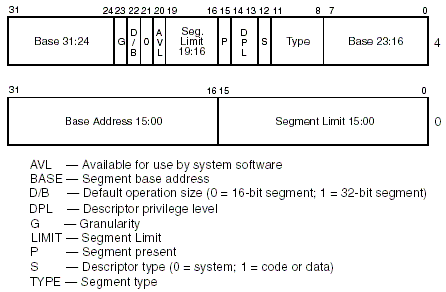
\includegraphics[width=9cm]{imagenes/gdt.png}
\end{center}
\end{figure}

En éste ejercicio vamos a definir 4 segmentos, cada uno con su entrada en la GDT.

\subparagraph*{Entrada 1}
\begin{itemize}
	
    \item $.base_{0-15}$ = 0,

    \item $.base_{23-16}$ = 0,
    \item $.base_{31-24}$ = 0,
    
El segmento empieza en la dirección de memoria 0.
        
    \item $.limit_{0-15}$ = 0xDCFF,
    \item $.limit_{16-19}$ = 0x2;

733 MB = 187648 bloques de 4 KB.
\\ El máximo offset que queremos utilizar es 187648 - 1 = 0x2DCFF 
    
    \item .type = 8
        
Será un segmento de código $Execute-Only$.
        
    \item .s  = 1
        
Código/Datos \fixme{explicar que significa esto}
        
    \item .dpl = 0
        
Este segmento tendrá nivel de privilegio 0.

    \item .p = 1
        
Este segmento estará presente en memoria.  \fixme{asi se expresa?}
    
    \item .avl = 0
        
A disposición del programador.


    \item .l = 0
        
Sólo va en 1 cuando estás en modo IA-32e \fixme{no esta en nuestro dibujo}

    \item .db = 1
        
Siginifica que vamos a trabajar en 32 bits. \fixme{especificamente?}

    \item .g = 1

Nuestro límite lo vamos a expresar con una granularidad de 4KB en vez de 1B. Es decir, vamos a poder direccionar (limite - 1) * 4K bytes.

\end{itemize}

\subparagraph*{Entrada 2}

Se diferencia de la entrada 1 en que el campo $dpl$ - el nivel de privilegio - se pone en 3.

\subparagraph*{Entrada 3}

Se diferencia de la entrada 1 en que el campo $type$ se pone en 2 - $Read-Write$.

\subparagraph*{Entrada 4}

Se diferencia de la entrada 3 en que el campo $dpl$ se pone en 3.

% Ejercicio 1 - b)
\paragraph{Modo Protegido}\label{subsubsec:ej1-b}
Completar el código necesario para pasar a modo protegido y setear la pila del
kernel en la dirección 0x27000.
\hruler
\fixme{Respuesta}

% Ejercicio 1 - c)
\paragraph{GDT - Área de Memoria}\label{subsubsec:ej1-c}
Declarar un segmento adicional que describa el área de la pantalla en memoria
que pueda ser utilizado sólo por el kernel.
\hruler
\fixme{Respuesta}

% Ejercicio 1 - d)
\paragraph{Limpiar la pantalla}\label{subsubsec:ej1-d}
Escribir una rutina que se encargue de limpiar la pantalla y pintar el area de
el mapa un fondo de color (sugerido verde). Para este ejercicio se debe escribir
en la pantalla usando el segmento declarado en el punto anterior (para los
próximos ejercicios se accederá a la memoria de vídeo por medio del segmento de
datos de 773MB).

Nota: La GDT es un arreglo de gdt entry declarado sólo una vez como gdt. El
descriptor de la GDT en el código se llama GDT DESC.
\hruler
\fixme{Respuesta}
